\chapter{Erzeugung der konjunktiven Normalform}
\label{chp:knf}

Der einfachste Weg eine konjunktive Normalform zu erzeugen, die erfüllbarkeitsäquivalent zu \glos{sha256} ist, führt vermutlich über die Verwendung vom \acr{cbmc}
(siehe Abschnitt \ref{sec:cbmc}). \acr{cbmc} erzeugt zur Verifikation von Aussagen über C-Programmcode eine konjunktive Normalform und übergibt diese direkt
an einen SAT-Solver (siehe Abschnitt \ref{sec:satsolver}). Es besteht jedoch auch die Möglichkeit die generierte konjunktive Normalform im DIMACS-Format auszugeben,
so dass ein C-Programm automatisch übersetzt werden kann. Dabei gehen jedoch jegliche Informationen über den Aufbau und die Bedeutung einzelner Literale verloren,
so dass es nicht möglich ist, erworbenes Wissen über Literale einzelnen Berechnungen zuzuordnen. Ausgehend von der Addition, die in der Kompressionsfunktion von
\glos{sha256} am häufigsten verwendet wird, ist es somit nicht möglich, erworbenes Wissen darüber zuzuordnen und auf alle weiteren Additionen zu übertragen.
Außerdem ist es nicht möglich Einfluss auf die Anzahl und Verwendung der Literale zu nehmen. Für einen Addierer liegt die Entscheidung somit bei \acr{cbmc},
wie dieser realisiert wird und ob und wie viele zusätzliche Literale verwendet werden. Das eine Extrem wäre die Verwendung eines Carry-Ripple-Addieres, dessen einzelne
Volladdierer in Gatter zerlegt werden, die dann einzeln in die konjunktive Normalform überführt werden. Das führt zu vergleichsweise vielen Literalen mit wenig
kurzen Klauseln. Das andere Extrem wäre der Versuch, eine konjunktive Normalform zu erzeugen, die ausschließlich Literale für die Summanden und die Summe erzeugt.
Dabei entstehen jedoch vergleichsweise viele lange Klauseln.

Um sowohl Kontrolle über die Erzeugung der konjunktiven Normalform zu bekommen als auch Informationen zu sammeln um eine Analyse zu ermöglichen, wird ein Programm
erstellt, dass das Entwurfsmuster "`Besucher"' \cite[301]{visitor} verwendet. Besucher sind dabei Instanzen von Klassen, die unterschiedlichste Aufgaben erfüllen können.
Eine Aufgabe kann es dabei sein, die konjunktive Normalform zu erzeugen während eine andere Aufgabe das Zählen von Literalen und Klauseln sein kann.
Besucht wird dabei eine Struktur, deren Objekte das Verhalten von \glos{sha256} beschreiben. Die Objekte der Struktur werden im Folgenden als Modul bezeichnet.
Ein Modul kann sowohl die vollständige Kompressionsfunktion von \glos{sha256} sein, als auch ein kleiner Baustein wie ein Halbaddierer. Dabei kann ein Modul
auch andere Module verwenden. Es zeigt sich, dass acht grundlegende Module ausreichen um \glos{sha256} vollständig zu beschreiben. Diese werden in den Abschnitten
\ref{sec:knf:addierer} bis \ref{sec:knf:sig} erläutert. Alle weiteren Module setzen sich aus diesen zusammen und werden in Abschnitt \ref{sec:knf:module} erläutert.

Alle notwendigen allgemeinen Funktionen für ein Modul sind in einer Basisklasse hinterlegt, von der jedes konkrete Modul erben muss. Ein konkretes Modul wird
dadurch realisiert, dass die bis dato rein virtuelle Funktion create(Collector* collector) implementiert wird. Über diese Funktion wird der Besucher in das Modul
übergeben, dessen Basisklasse im Folgenden Collector genannt wird, da dieser Informationen über die besuchten Module sammelt. Der Collector stellt 2 virtuelle
Funktionen bereit, die ein konkreter Collector implementieren kann.
\begin{description}
  \item[newModul(unsigned level, const char* name, Modul* modul)] muss von jedem Modul aufgerufen werden und dient der Registrierung im Collector.
       Übergeben wird dabei ein selbstgewähltes Level und ein eindeutiger Name. Das Level muss dabei immer höher sein, als alle Level der im Modul
       benutzen Module, so dass Module eines Levels keine gemeinsamen Literale verwenden. Der Name dient als Identifizierung um eine mehrfache
       Verwendung eines Moduls zu erkennen und gelerntes Wissen zuordnen zu können. Als weiterer Parameter wird noch ein Pointer auf das Modul
       selbst übergeben, so dass der Collector bei Bedarf weitere Informationen abrufen kann.
  \item[create(bool xOR, const std::vector<CMSat::Lit>\& vars)] kann von einem Modul mehrfach aufgerufen werden, um Klauseln zu generieren.
       Im Fall von \glos{sha256} wird diese Funktion nur von den acht grundlegenden Modulen aufgerufen. Alle weiteren Module setzen sich aus
       diesen zusammen und reichen den Collector lediglich weiter. Der erste Paramter gibt an, ob es sich um eine normale Klausel handelt,
       deren Literale durch ein OR verknüpft sind, oder ob es sich um eine Klausel handelt deren Literale durch ein XOR verknüpft sind.
       Ein SAT-Solver wie CryptoMiniSat kann XOR-Klauseln direkt verarbeiten. Für SAT-Solver ohne Unterstützung der XOR-Klauseln ist eine
       Transformation in OR-Klauseln einfach möglich. Eine Transformation in die andere Richtung würde das Sammeln und Analysieren der
       OR-Klauseln erfordern und wäre dadurch wesentlich aufwendiger.
\end{description}
Die für die Analyse notwendigen konkreten Collectoren werden in Kapitel \ref{chp:analyse} erläutert.

Als Hilfsmittel für die Generierung der Klauseln wird die Klasse ClauseCreator genutzt. Die Verwendung ist in einem Beispiel in Abbildung \ref{fig:clausecreator} dargestellt.
Initialisiert wird der ClauseCreator durch die Übergabe des Collectors, an den die Klauseln übergeben werden sollen. Im Anschluss werden die Nummern der Literale gesetzt.
Dadurch ist es möglich mit diesen Literalen beliebig viele Klauseln zu erzeugen, wobei nur noch die Polarität angegeben werden muss. 0 führt zu einer Negation während
das Makro CC\_DC ein Dont-Care signalisiert und das Literal in der Klausel unterdrückt wird.
\begin{figure}[!h]
  \centering
  \begin{minipage}[c]{7.5cm}
    \begin{lstlisting}[language=c]
	ClauseCreator cc(collector);
	cc.setLiterals(4,     0,     1,     2,     3);
	cc.printClause(4,     0,     1, CC_DC, CC_DC);
	cc.printClause(4,     1,     0,     1,     0);
	cc.printClause(4, CC_DC, CC_DC,     1, CC_DC);
    \end{lstlisting}
  \end{minipage}
  \begin{minipage}[c]{2cm}
    ~~~~~~~~~~~~$ \Rightarrow $   
  \end{minipage}
  \begin{minipage}[c]{2cm}
    \begin{align*}
      & (\overline{0} \vee 1) ~ \wedge \\
      & (0 \vee \overline{1} \vee 2 \vee \overline{3}) ~ \wedge \\
      & (2) \nonumber
    \end{align*}
  \end{minipage}
  \caption{Verwendung des ClauseCreators}
  \label{fig:clausecreator}
\end{figure}

Um die Funktion aller Module sicherzustellen, werden diese mit MinUnit \cite{minunit} getestet. MinUnit ist eine minimale Testumgebung und
wurde ursprünglich für den Test von C-Programmen entwickelt. Da es unter der MIT-Lizenz veröffentlicht wurde kann es ohne Einschränkungen
direkt in den Programmcode eingebunden und angepasst werden. Ausgeliefert wird MinUnit in einer einzigen Header-Datei. Das führt zu einem
Problem wenn der Linker mehrere Objekt-Dateien zusammenführt, da MinUnit mehrfach eingebunden wurde. Um dieses Problem zu vermeiden, wird
der Programmcode von MinUnit in eine Header- und eine Quelltext-Datei aufgeteilt.

Für die Erzeugung einer potentiell minimalen konjunktiven Normalform wird im ersten Schritt das Programm eqntott verwendet. Mit Hilfe von eqntott
ist es möglich, boolsche Gleichungen in eine Wahrheitstabelle zu überführen. Da das Eingabeformat weder den XOR- noch den Gleichheits-Operator unterstützt,
müssen diese beiden Operatoren in der Eingabedatei selbst definiert werden. Ein binärer XOR-Operator entspricht dabei einem negierten Gleichheits-Operator.
Die Definitionen in Abbildung \ref{fig:gatter_equations_head} werden bei allen Berechnungen in den nächsten Abschnitten verwendet.
\begin{figure}[!h]
  \centering
  \begin{minipage}[c]{14.5cm}
    \begin{lstlisting}[]
  #define xor(a,b) ((a)&!(b) | !(a)&(b))
  #define eq(a,b) ((a)&(b) | !(a)&!(b))
    \end{lstlisting}
  \end{minipage}
  \caption{Gattergleichungen - Kopf}
  \label{fig:gatter_equations_head}
\end{figure}

Die ermittelte Wahrheitstabelle kann jedoch nicht direkt in eine konjunktive Normalform überführt werden. Sie enthält alle Einträge die die boolsche Gleichung erfüllen
und ist mit großer Wahrscheinlichkeit nicht minimal. Für die konjunktive Normalform werden alle Einträge benötigt, die die boolsche Gleichung nicht erfüllen. Um diese zu
generieren wäre es möglich, die boolsche Gleichung entsprechend anzupassen. Am Beispiel eines 4-Bit-Addierers zeigt sich jedoch, dass das Ergebnis wesentlich größer sein kann.
Ein 4-Bit-Addierer hat $2^4$ mögliche Ergebnisse. Jedes dieser Ergebnisse lässt sich aus $2^4$ unterschiedlichen Summanden gewinnen. Es gibt somit $(2^4)^2 = 256$
erfüllende Belegungen. Im Gegensatz dazu stehen bei jedem möglichen Ergebnis $2^4 \cdot (2^4-1)$ mögliche Kombinationen von Summanden die nicht zum Ergebnis führen.
Die nicht erfüllenden Belegungen belaufen sich somit auf $(2^4)^2 \cdot ((2^4)-1) = 3840$. Da diese Wahrheitstabelle nur als Zwischenergebnis und Eingabe für
Espresso (siehe Abschnitt \ref{sec:espresso}) verwendet werden soll, werden deshalb die erfüllenden Belegungen generiert.

Die Wahrheitstabelle wird im zweiten Schritt an Espresso übergeben. Nachdem Espresso die Wahrheitstabelle eingelesen hat führt der Parameter -epos dazu,
dass die erfüllenden Belegungen in nicht-erfüllende überführt werden. Diese Belegungen werden von Espresso minimiert. Durch den Parameter -Dexact wird
eine minimale Anzahl an Belegungen garantiert. Das führt jedoch nur bei Problemen mit wenig Variablen zu einer Lösung, hat sich jedoch in den vorliegenden
Fällen bewährt.

Die minimierten nicht-erfüllenden Belegungen gibt Espresso wieder in einer Wahrheitstabelle aus. Diese kann nun einfach in eine konjunktive Normalform überführt werden.
Abbildung \ref{fig:truetocnf} zeigt dafür ein Beispiel. Ist zum Beispiel die Belegung b=$1$ und c=$1$ gegeben, führt dies dazu, dass die Klausel
$ (\overline{b} \vee \overline{c}) $ zu $0$ evaluiert und die Formel nicht mehr erfüllbar ist,was genau dem gewünschten Verhalten entspricht.
\begin{figure}[!h]
  \centering
  \begin{tabular}{c|c|c|cp{0.5cm}cp{0.5cm}l}
    \hiderowcolors
    a & b & c & d &  & \\
    \cline{1-4}
    1 & 0 & - & 0 &  & $\Rightarrow$ &  & $ (\overline{a} \vee b \vee d) ~ \wedge $\\
    - & 0 & 0 & 1 &  & $\Rightarrow$ &  & $ (b \vee c \vee \overline{d}) ~ \wedge $\\
    0 & 0 & 0 & 0 &  & $\Rightarrow$ &  & $ (a \vee b \vee c \vee d) ~ \wedge $\\
    - & 1 & 1 & - &  & $\Rightarrow$ &  & $ (\overline{b} \vee \overline{c}) $\\
    \showrowcolors
  \end{tabular}
  \caption{Wahrheitstabelle -> Konjunktive Normalform}
  \label{fig:truetocnf}
\end{figure}

Nachdem das allgemeine Vorgehen erläutert wurde, werden in den folgenden Abschnitten die konkreten Ergebnisse für die einzelnen Kompontenten von \glos{sha256} vorgestellt.

\section{Gatter}
\label{sec:knf:gatter}

Grundlage für die Tseitin-Transformation (siehe Abschnitt \ref{sec:knf}) sollen in dieser Arbeit die Operatoren AND, OR und XOR bilden. Verwendet werden sie jedoch
nur, falls sie in einem Modul eine direkte Beziehung zwischen Eingangs- und Ausgang-Literalen definieren, da sonst zusätzliche Literale eingefügt werden müssen.
Die Boolesche Gleichungen für die drei Operatoren sind in Abbildung \ref{fig:gatter_equations} dargestellt. a und b werden als Literale für die Eingänge verwendet
und r steht für den Ausgang (das Resultat).

\begin{figure}[!h]
  \centering
  \begin{minipage}[c]{4.85cm}
    \begin{lstlisting}[]
  NAME = AND;
  INORDER = r_out a_in b_in;
  OUTORDER = z;

  z = eq(r_out, (a_in & b_in));
    \end{lstlisting}
  \end{minipage}
  \begin{minipage}[c]{4.85cm}
    \begin{lstlisting}[]
  NAME = OR;
  INORDER = r_out a_in b_in;
  OUTORDER = z;

  z = eq(r_out, (a_in | b_in));
    \end{lstlisting}
  \end{minipage}
  \begin{minipage}[c]{5.1cm}
    \begin{lstlisting}[]
  NAME = XOR;
  INORDER = r_out a_in b_in;
  OUTORDER = z;

  z = eq(r_out, xor(a_in, b_in));
    \end{lstlisting}
  \end{minipage}
  \caption{Gatter - Gleichungen}
  \label{fig:gatter_equations}
\end{figure}

Nach der Verwendung von eqntott und Espresso ergeben sich aus den Booleschen Gleichungen die konjunktiven Normalformen in Abbildung \ref{fig:gatter_cnf}.
Diese decken sich mit den Angaben auf Wikipedia \cite{wiki:tseitin}. Für die Negation der Operatoren reicht es aus, das Ergebnisliteral r zu invertieren.

\begin{figure}[!h]
  \centering
  \begin{minipage}[l]{4.65cm}
    \underline{AND}\\
    $ (\overline{r} \vee a) ~ \wedge $\\
    $ (\overline{r} \vee b) ~ \wedge $\\
    $ (r \vee \overline{a} \vee \overline{b}) $\\
    ~
  \end{minipage}
  \begin{minipage}[l]{4.65cm}
    \underline{OR}\\
    $ (r \vee \overline{a}) ~ \wedge $\\
    $ (r \vee \overline{b}) ~ \wedge $\\
    $ (\overline{r} \vee a \vee b) $\\
    ~
  \end{minipage}
  \begin{minipage}[l]{4.3cm}
    \underline{XOR}\\
    $ (\overline{r} \vee \overline{a} \vee \overline{b}) ~ \wedge $\\
    $ (r \vee a \vee \overline{b}) ~ \wedge $\\
    $ (r \vee \overline{a} \vee b) ~ \wedge $\\
    $ (\overline{r} \vee a \vee b) $
  \end{minipage}
  \caption{Gatter - Konjunktive Normalformen}
  \label{fig:gatter_cnf}
\end{figure}

Während es bei den Operatoren AND und OR gelungen ist, Don't-Care Literale zu identifizieren und für eine Vereinfachung zu nutzen, ist dies bei dem XOR-Operator
nicht möglich. Jede einzelne Änderung eines beliebigen Eingangsliterals führt zu einer Änderung des Ausgangssignals. Genau die Hälfte der möglichen Belegungen
ist somit nicht erfüllbar und muss in die konjunktive Normalform mit aufgenommen werden. Allgemein gilt, dass bei einem XOR mit n Eingängen $ 2^{n} $ Klauseln
mit jeweils $ (n + 1) $ Literalen notwendig sind. Die Klauselmenge wächst exponentiell im Bezug zur Anzahl der Eingänge.

CryptoMiniSat (siehe Abschnitt \ref{sec:satsolver}) ist in der Lage, neben normalen Klauseln (Disjunktion) auch Klauseln zu berücksichtigen, deren Literale
mit dem XOR-Operator verknüpft sind. Genau wie normale Klauseln müssen sie für die Erfüllbarkeit zu $1$ evaluiert werden. Damit lässt sich das exponentielle
Wachstum der Klauselmenge umgehen. Für ein XOR mit n Eingängen ist nur noch eine Klausel mit $ (n + 1) $ Literalen notwendig. Abbildung \ref{fig:gatter_cnf_xor}
zeigt die Klausel für den XOR-Operator mit zwei und drei Eingängen.
\begin{figure}[!h]
  \centering
  \begin{minipage}[l]{1cm}
    ~\\
    ~
  \end{minipage}
  \begin{minipage}[l]{2.5cm}
    Zwei Eingänge:\\
    Drei Eingänge:
  \end{minipage}
  \begin{minipage}[l]{3cm}
    $ (\overline{r} \veebar a \veebar b) $\\
    $ (\overline{r} \veebar a \veebar b \veebar c) $
  \end{minipage}
  \caption{Gatter - XOR}
  \label{fig:gatter_cnf_xor}
\end{figure}

Abschließend wird noch ein Operator für die Negation (NOT) benötigt. Um daraus einen Gleichheits-Operator (EQ) zu machen reicht es aus, das Ergebnisliteral r zu invertieren.
Realisiert wird die Negation durch eine XOR-Klausel mit zwei Literalen (siehe Abbildung \ref{fig:gatter_not_cnf}). Diese wird nur dann zu $1$ evaluiert, wenn
a und r unterschiedlich sind, was genau der Negation entspricht. Falls XOR-Klauseln nicht unterstützt werden, lässt sich die Negation mit zwei Klauseln à zwei
Literalen realisieren, wie ebenfalls in der Abbildung dargestellt. Auch diese konjunktive Normalform deckt sich mit der Angabe auf Wikipedia \cite{wiki:tseitin}.
\begin{figure}[!h]
  \centering
  \begin{minipage}[l]{1cm}
    ~\\
    ~
  \end{minipage}
  \begin{minipage}[l]{2.5cm}
    \underline{Ohne XOR}\\
    $ (r \vee a) ~ \wedge $\\
    $ (\overline{r} \vee \overline{a}) $
  \end{minipage}
  \begin{minipage}[l]{2.5cm}
    \underline{Mit XOR}\\
    $ (r \veebar a) $\\
    ~
  \end{minipage}
  \caption{Gatter - NOT - Konjuktive Normalform}
  \label{fig:gatter_not_cnf}
\end{figure}
\section{Addierer}
\label{sec:knf:addierer}

Grundlage für die modulare 32-Bit Addition sind der Halbaddierer, der Volladdierer und der Mod2 Addierer (siehe Abschnitt \ref{sec:grundlagen_add}).

Wie auch für die Gatter im Abschnitt vorher wird für den Halbaddierer eine boolsche Gleichungen erstellt (siehe Abbildung \ref{fig:halfadder_eqn}).
Diese entspricht genau den Gattern in Abbildung \ref{fig:halfadder}.
\begin{figure}[!h]
  \centering
  \begin{lstlisting}[]
  NAME = HalfAdder;
  INORDER = c_out s_out a_in b_in;
  OUTORDER = z;

  z = eq(s_out, xor(a_in, b_in)) & eq(c_out, a_in & b_in);
  \end{lstlisting}
  \caption{Halbaddierer - Gleichung}
  \label{fig:halfadder_eqn}
\end{figure}

Nach der Verwendung von eqntott und Espresso ergibt sich aus der boolenschen Gleichung die konjunktive Normalform in Abbildung \ref{fig:halfadder_cnf} (linke Seite).
eqntott und Espresso unterstützen jedoch keine XOR-Klauseln, weshalb ein manueller Versuch unternommen wird, diesen Vorteil zu nutzen. Das Ergebnis ist in Abbildung
\ref{fig:halfadder_cnf} (rechte Seite) dargestellt und besteht aus dem AND- und dem XOR-Gatter. Die Klauselmenge kann so von sechs auf vier Klauseln reduziert werden.
Diese Lösung bietet sich jedoch nur an, wenn die XOR-Klausel auch direkt verwendet werden kann. Wird sie in normale Klauseln umgewandelt, stehen im Ergebnis sieben
Klauseln. Das ist eine mehr als in der Lösung von Espresso.
\begin{figure}[!h]
  \centering
  \begin{minipage}[l]{5cm}
    ~~~~~~~~\underline{Ohne XOR}\\
    $ (\overline{s} \vee a \vee b) ~ \wedge $\\
    $ (\overline{c} \vee \overline{s}) ~ \wedge $\\
    $ (\overline{c} \vee b) ~ \wedge $\\
    $ (c \vee \overline{a} \vee \overline{b}) ~ \wedge $\\
    $ (s \vee a \vee \overline{b}) ~ \wedge $\\
    $ (s \vee \overline{a} \vee b) $
  \end{minipage}
  \begin{minipage}[l]{5cm}
    ~~~~~~~~\underline{Mit XOR}\\
    \underline{Übertrag - AND}\\
    $ (\overline{c} \vee a) ~ \wedge $\\
    $ (\overline{c} \vee b) ~ \wedge $\\
    $ (c \vee \overline{a} \vee \overline{b}) ~ \wedge $\\
    \underline{Summe - XOR}\\
    $ (\overline{s} \veebar a \veebar b) $
  \end{minipage}
  \caption{Halbaddierer - Konjuktive Normalform}
  \label{fig:halfadder_cnf}
\end{figure}

\begin{figure}[!h]
  \centering
  \lstset{moredelim=**[is][\color{blue}]{@}{@}, moredelim=**[is][\bfseries]{§}{§}}
  \begin{lstlisting}[]
  NAME = FullAdder;
  INORDER = c_out §@s_out@§ a_in b_in c_in;
  OUTORDER = z;

  z = §@eq(s_out, xor(xor(a_in, b_in), c_in)) &@§ eq(c_out, (a_in & b_in) | (xor(a_in, b_in) & c_in));
  \end{lstlisting}
  \caption{Volladdierer - Gleichung}
  \label{fig:fulladder_qen}
\end{figure}

\begin{figure}[!h]
  \centering
  \begin{minipage}[l]{5cm}
    ~~~~~~~~\underline{Ohne XOR}\\
    $ (s \vee \overline{a} \vee \overline{b} \vee \overline{c}) ~ \wedge $\\
    $ (\overline{s} \vee a \vee b \vee c) ~ \wedge $\\
    $ (o \vee \overline{a} \vee \overline{b}) ~ \wedge $\\
    $ (\overline{o} \vee a \vee b) ~ \wedge $\\
    $ (o \vee s \vee \overline{c}) ~ \wedge $\\
    $ (\overline{o} \vee \overline{s} \vee c) ~ \wedge $\\
    $ (\overline{s} \vee a \vee \overline{b} \vee \overline{c}) ~ \wedge $\\
    $ (\overline{s} \vee \overline{a} \vee b \vee \overline{c}) ~ \wedge $\\
    $ (s \vee a \vee \overline{b} \vee c) ~ \wedge $\\
    $ (s \vee \overline{a} \vee b \vee c) $
  \end{minipage}
  \begin{minipage}[l]{5cm}
    ~~~~~~~~\underline{Mit XOR}\\
    \underline{Übertrag}\\
    $ (o \vee \overline{a} \vee \overline{b}) ~ \wedge $\\
    $ (\overline{o} \vee a \vee b) ~ \wedge $\\
    $ (o \vee \overline{a} \vee \overline{c}) ~ \wedge $\\
    $ (o \vee \overline{b} \vee \overline{c}) ~ \wedge $\\
    $ (\overline{o} \vee a \vee c) ~ \wedge $\\
    $ (\overline{o} \vee b \vee c) ~ \wedge $\\
    \underline{Summe - XOR}\\
    $ (\overline{s} \veebar a \veebar b \veebar c) $\\
    ~
  \end{minipage}
  \caption{Volladdierer - Konjuktive Normalform}
  \label{fig:fulladder_cnf}
\end{figure}

nur carry ripple addierer\\
vergleich addierer höherer ebene\\
halbaddierer\\
volladdierer\\
mod2addierer\\
~\\
bei erster ebene: xor support: cryptominisats xor nutzen. ansonsten espresso
\section{Addierer (Konstante)}
\label{sec:knf:konstadd}

\TODO{erledigen}

wie addierer aber 32 literale direkt weggekürzt\\
abhängig von der konstante
\section{Choose (CH)}
\label{sec:knf:ch}

Die Choose-Funktion kann durch zwei AND-Gatter und ein XOR-Gatter realisiert werden. Als Alternative für das XOR-Gatter wird auch ein OR-Gatter berücksichtigt.
Bei Verwendung der Gatter müssen 2 zusätzliche Literale eingefügt werden, die das Ergebnis der beiden AND-Gatter enthalten, so dass insgesamt 6 Literale benötigt werden.
Für die AND-Gatter werden jeweils drei Klauseln benötigt. Das XOR-Gatter benötigt eine XOR-Klausel oder vier normale Klauseln, während das OR-Gatter drei Klauseln benötigt.
Je nach Realisierung ergeben sich damit zehn, neun oder sieben Klauseln.

Nach den Erfolgen in den beiden vorhergehenden Abschnitten wird für die Choose-Funktion ebenfalls eine Boolesche Gleichung erstellt (siehe Abbildung \ref{fig:choose_eqn}).
Im Gegensatz zu den Addierern ist das Ergebnis des XOR-Gatters nicht direkt von Eingaben abhängig, sondern von anderen Gattern. Damit lässt sich das XOR-Gatter nicht
ausgliedern und separat betrachten, so dass nur die vollständige Boolesche Gleichung genutzt wird.
\begin{figure}[!h]
  \centering
  \begin{lstlisting}[]
  NAME = CH;
  INORDER = r_out a_in b_in c_in;
  OUTORDER = z;

  z = eq(r_out, xor(a_in & b_in, !a_in & c_in));
  \end{lstlisting}
  \caption{Choose - Gleichung}
  \label{fig:choose_eqn}
\end{figure}

Aus der Berechnung von eqntott und Espresso ergibt sich die konjunktive Normalform in Abbildung \ref{fig:choose_cnf}.
Vier Klauseln reichen aus, um die Choose-Funktion zu beschreiben.
\begin{figure}[!h]
  \centering
  \begin{minipage}[l]{2cm}
    $ (r \vee \overline{a} \vee \overline{b}) ~ \wedge $\\
    $ (\overline{r} \vee \overline{a} \vee b) ~ \wedge $\\
    $ (r \vee a \vee \overline{c}) ~ \wedge $\\
    $ (\overline{r} \vee a \vee c) $
  \end{minipage}
  \caption{Choose - Konjuktive Normalform}
  \label{fig:choose_cnf}
\end{figure}

In Tabelle \ref{fig:choose_literalclausecount} sind die unterschiedlichen Lösungen gegenübergestellt.
Die Choose-Funktion wird bitweise auf einer 32 Bit breiten Binärzahl angewendet. Jedes Bit der Eingabe wird dabei nur einmal genutzt.
Die einzelnen Berechnungen sind somit unabhängig, wodurch sich die Gesamtanzahl der Literale und Klauseln aus der Multiplikation mit 32 ergibt.
\begin{table}[!h]
  \centering
  \begin{tabular}{l|r|r}
    \hiderowcolors
    \textbf{Lösung}        & \textbf{Choose} & \textbf{Gesamt} \\
    \hline
    \showrowcolors
    Gatter                 &  6 -  10 & 192 - 320 \\
    Gatter mit OR          &  6 - ~~9 & 192 - 288 \\
    Gatter mit XOR         &  6 - ~~7 & 192 - 224 \\
    eqntott \& Espresso    &  4 - ~~4 & 128 - 128 \\
  \end{tabular}
  \caption{Choose - Literale und Klauseln}
  \label{fig:choose_literalclausecount}
\end{table}

Das Ergebnis zeigt, dass es nicht notwendig ist, unterschiedliche Lösungen bereitzustellen. Egal ob eine XOR-Unterstützung gegeben ist oder nicht,
ist die von eqntott und Espresso ermittelte Lösung optimal und wird implementiert.
\section{Majority (MAJ)}
\label{sec:knf:maj}

Die Majority-Funktion ist ähnlich aufgebaut wie die Choose-Funktion und enthält ein AND-Gatter mehr. Für die auf den Gattern basierte Lösung sind somit drei zusätzliche
Literale notwendig. Anstatt vier werden sieben Literale benötigt. Für die AND-Gatter werden jeweils drei Klauseln benötigt. Für die XOR- bzw. OR-Funktion wird jeweils
ein Gatter mit drei Eingängen herangezogen um zumindest hier ein zusätzliches Literals zu vermeiden. Das XOR-Gatter benötigt eine XOR-Klausel oder acht normale Klauseln
während das OR-Gatter vier Klauseln benötigt. Je nach Realisierung ergeben sich damit siebzehn, dreizehn oder zehn Klauseln.

Gegenübergestellt wird die Lösung von eqntott und Espresso die sich aus der Booleschen Gleichung in Abbildung \ref{fig:majority_eqn} ergibt.
\begin{figure}[!h]
  \centering
  \begin{lstlisting}[]
  NAME = MAJ;
  INORDER = r_out a_in b_in c_in;
  OUTORDER = z;

  z = eq(r_out, xor(xor(a_in & b_in, a_in & c_in), b_in & c_in));
  \end{lstlisting}
  \caption{Majority - Gleichung}
  \label{fig:majority_eqn}
\end{figure}

Die ermittelte konjunktive Normalform ist in Abbildung \ref{fig:majority_cnf} aufgeführt.
Sechs Klauseln reichen aus um die Majority-Funktion zu beschreiben.
\begin{figure}[!h]
  \centering
  \begin{minipage}[l]{2cm}
    $ (r \vee \overline{a} \vee \overline{b}) ~ \wedge $\\
    $ (\overline{r} \vee a \vee b) ~ \wedge $\\
    $ (r \vee \overline{a} \vee \overline{c}) ~ \wedge $\\
    $ (r \vee \overline{b} \vee \overline{c}) ~ \wedge $\\
    $ (\overline{r} \vee a \vee c) ~ \wedge $\\
    $ (\overline{r} \vee b \vee c) $
  \end{minipage}
  \caption{Majority - Konjuktive Normalform}
  \label{fig:majority_cnf}
\end{figure}

In Tabelle \ref{fig:majority_literalclausecount} sind die unterschiedlichen Lösungen gegenübergestellt.
Genau wie die Choose-Funktion wird die Majority-Funktion bitweise auf einer 32 Bit breiten Binärzahl angewendet. Jedes Bit der Eingabe wird dabei nur einmal genutzt.
Die einzelnen Berechnungen sind somit unabhängig wodurch sich die Gesamtanzahl der Literale und Klauseln aus der Multiplikation mit 32 ergibt.
\begin{table}[!h]
  \centering
  \begin{tabular}{l|r|r}
    \hiderowcolors
    \textbf{Lösung}        & \textbf{Majority} & \textbf{Gesamt} \\
    \hline
    \showrowcolors
    Gatter                 &  7 -  17 & 224 - 544 \\
    Gatter mit OR          &  7 -  13 & 224 - 416 \\
    Gatter mit XOR         &  7 -  10 & 224 - 320 \\
    eqntott \& Espresso    &  4 - ~~6 & 128 - 192 \\
  \end{tabular}
  \caption{Majority - Literale und Klauseln}
  \label{fig:majority_literalclausecount}
\end{table}

Auch dieses Ergebnis zeigt, dass es nicht notwendig ist, unterschiedliche Lösungen bereitzustellen.
Egal ob eine XOR-Unterstützung gegeben ist oder nicht, ist die von eqntott und Espresso ermittelte Lösung optimal und wird implementiert.
\section{Sigma-Familie (SIG)}
\label{sec:knf:sig}

Im Gegensatz zu den Funktionen in den vorhergehenden Abschnitten wird bei den Sigma-Funktionen ausschließlich das XOR-Gatter verwendet.
Während bisher mehrere Eingaben verrechnet wurden, wird bei den Sigma-Funktionen nur eine einzelne Eingabe verwendet, deren
einzelne Bits Verwendung in bis zu drei unterschiedlichen Ausgabebits finden. Da jedes Ausgabebit direkt durch ein XOR-Gatter aus den
Eingabebits berechnet wird, sind keine zusätzlichen Literale notwendig. Aus 32 Eingabebits und 32 Ausgabebits ergeben sich 64 Literale.

Bei Verwendung der XOR-Klauseln reicht eine Klausel für jedes Ausgabebit aus, unabhängig davon ob das Ausgabebit aus zwei oder drei
Eingangsbits berechnet wird. Anders ist es bei fehlender XOR-Unterstützung. Ein XOR mit drei Eingängen benötigt acht Klauseln während
ein XOR mit zwei Eingängen vier Klauseln benötigt. Bei den $ \Sigma $-Funktionen kommt dieser Unterschied nicht zum tragen, da generell
drei Eingabebits für jedes Ausgabebit herangezogen werden. Es ergeben sich 256 Klauseln. Anders verhält es sich bei den $ \sigma $-Funktionen.
Durch die Verschiebung nach rechts werden 3 bzw. 10 Eingangsbits nur zwei mal berücksichtigt. Die entstehende $0$ hat keinen Einfluss auf das
Ergebnis einer XOR-Operation und kann ignoriert werden. Es ergeben sich deshalb nur 244 bzw. 216 Klauseln. Eine Übersicht ist in Tabelle
\ref{fig:sigma_literalclausecount} dargestellt.
\begin{table}[!h]
  \centering
  \begin{tabular}{l|r|r|r|r}
    \hiderowcolors
    Funktion        & $ \sigma_0 $ & $ \sigma_1 $ & $ \Sigma_0 $ & $ \Sigma_1 $ \\
    \hline
    Gatter ohne XOR &     64 - 244 &     64 - 216 &     64 - 256 &     64 - 256 \\
    \hline
    Gatter mit XOR  &    64 - ~~32 &    64 - ~~32 &    64 - ~~32 &    64 - ~~32 \\
    \showrowcolors
  \end{tabular}
  \caption{Sigma - Literale und Klauseln}
  \label{fig:sigma_literalclausecount}
\end{table}

Wie auch für den Addierer, führt der Versuch die vier Funktionen als Wahrheitstabelle auszugeben und mit Espresso zu optimieren zu keinem Ergebnis.
\section{Übergeordnete Module}
\label{sec:knf:module}

Die acht grundlegenden Module aus den vorhergehenden Abschnitten werden in diesem Abschnitt genutzt,
um hierarchisch die vollständige Kompressionsfunktion von \glos{sha256} zu erzeugen. Eine einfache Lösung wäre es,
jeweils ein Modul für die Rundenfunktion und für die Erweiterung der Eingabe zu Erstellen. Diese werden
im Modul für die Kompressionsfunktion dann 64 bzw. 48 mal eingebunden. Das löst zwar die Generierung der konjunktiven
Normalform, ist jedoch für eine Analyse unter Umständen zu grob. Sollte es gelingen, Wissen mit CryptoMiniSat zu erwerben,
und einzelnen Modulen zuzuordnen, müsste eine weitere Zuordnung innerhalb des Moduls per Hand erfolgen.

Um dieses Problem zu vermeiden, werden zunächst kleinere Module definiert. Abbildung \ref{fig:sha256M} zeigt auf der linken
Seite zwei Module die Bestandteil der Rundenfunktion sind und jeweils aus drei anderen Modulen bestehen. Interessant ist dabei,
dass A und E jeweils Eingang in zwei Module finden, deren Ergebnisse durch eine Addition wieder zusammengeführt werden. Die
Analyse dieser Rekonvergenzen ist besonders interessant und wird durch die beiden Module vereinfacht.
\begin{figure}[!h]
  \centering
  \begin{minipage}[l]{9.5cm}
    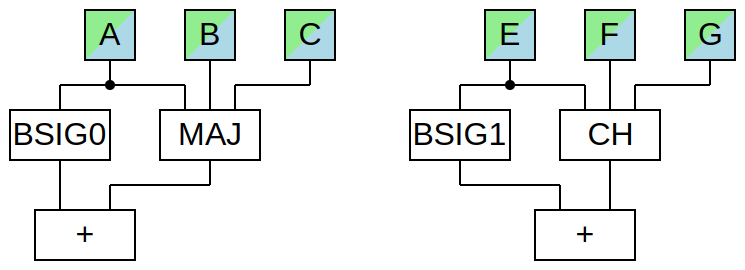
\includegraphics[scale=0.4]{images/sha256coreM}
  \end{minipage}
  \begin{minipage}[l]{3cm}
    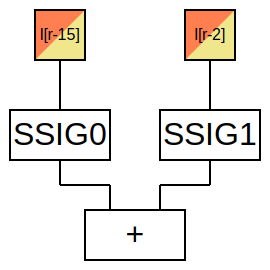
\includegraphics[scale=0.4]{images/sha256prepM}
  \end{minipage}    
  \caption{Erweiterte Module von \glos{sha256}}
  \label{fig:sha256M}
\end{figure}

Ein weiteres Modul ist Bestandteil der Erweiterung der Eingabe und in Abbildung \ref{fig:sha256M} auf der rechten Seite
dargestellt. Bei der Erweiterung der Eingabe werden vier Werte Addiert, wobei zwei davon zunächst durch die $ \sigma $-Funktionen
transformiert werden. Da es keine Rolle spielt, in welcher Reihenfolge die Addition durchgeführt wird, werden diese
beiden zunächst in einem eigenen Modul addiert. Da jedes Eingabebit der $ \sigma $-Funktionen Einfluss auf bis zu
drei Ausgabebits hat, könnten sich möglicherweise Rückschlüsse auf die jeweils anderen Eingabebits ziehen lassen.
Mit Hilfe dieses Moduls und weiteren Additionen, wird schließlich ein Modul für die vollständige Erweiterung der Eingabe
(siehe Abbildung \ref{fig:sha256prep}) erstellt. Die verbleibenden beiden Werte werden zunächst Addiert, um das Ergebnis
dann mit dem Ergebnis des Moduls zu addieren.

Die beiden erstgenannten Module werden ebenfalls zusammen mit weiteren Additionen genutzt, um ein Modul für die vollständige
Rundenfunktion (siehe Abbildung \ref{fig:sha256core}) zu realisieren. Außen vor bleibt dabei die Addition der Konstante.
Dadurch kann erworbenes Wissen auf alle 64 Runden angewendet werden, da es sich jedes Mal um das gleiche Modul handelt.
In einem weiteren Modul wird schließlich die Rundenfunktion mit der Addition der Konstante zusammengeführt.
Erworbenes Wissen, was auf der Konstante basiert, kann dadurch in diesem Modul gesammelt werden, falls es sich in einem
zweiten Schritt als allgemeingültig erweist.

Abschließend werden die genannten Module in einem Modul für die vollständige Rundenfunktion genutzt. Zusätzlich erfolgt in
diesem Modul auch die \ref{fig:sha256single} Addtion \TODO{erledigen}

Erweiterungsfunktion\\
Rundenfunktion\\
Rundenfunktion + Konstante\\
\glos{sha256} als ganzes: wissen hinzufügen und mehrfache verwendung bei bitcoin\\
~\\
Rekonvergenzen bei ersten beiden finden.\\
~\\
baum\\
hierarchie durch level:\\
subaddierer bekommen ihre ebene: 1 bis 4\\
module aus grafik ebene 10\\
11\\
20\\
21\\
sha als ganzes: 30\\
~\\
betrachtung der erweiterung als teil der runden 17 bis 64
\section{Vergleich mit CBMC}

\TODO{erledigen}